\documentclass[main.tex]{subfiles}

\begin{document}

% \textcolor{red}{Вводная лекция}

\section{Лекция 23.03.2021 (Донцов Е.В.)}

\subsection{Математическая модель EP3D (Enhanced pseudo-3D model)}

\includegraphics[width=\textwidth, page=73]{HF_slides_2021.pdf}

Далее рассмотрим псевдотрёхмерную модель.
Эта модель также относится к классу простых фундаментальных моделей, которые были разработаны в 80-х и 90-х годах, т.е. когда ещё не было широкодоступных больших вычислительных мощностей (другими словами, была необходимость произвести моделирование с использованием более простых подходов).

Про более сложные численные модели (planar3D ILSA и Biot) поговорим на следующих лекциях.

Важно, что на простых моделях можем многое изучить и можем понять, как будет вести себя более сложная модель.
\\

Целью псевдотрёхмерной модели является улучшение модели PKN.
Ранее обсуждали модель PKN (одномерная, постоянная высота).
Одномерность позволяла относительно легко анализировать уравнение, получить приближённые решения, делать какие-то оценки на пальцах.
У модели PKN реалистичная геометрия и она довольно часто реализуется на практике.
Примечание: у радиальной трещины геометрия не совсем реалистична, потому что в породе практически всегда есть слои, которые не учитываются этой моделью (она не может реализоваться в случае наличия слоёв в породе).
\\

Псевдотрёхмерная модель довольно часто реализуется на практике и является следующим шагом (после модели PKN) по сложности.
Она всё ещё одномерная.
\\

Давайте посмотрим, что включает в себя эта модель.

Теперь вместо полностью непроницаемых барьеров над и под разервуаром высоты $H$ будем рассматривать стресс барьеры с дополнительным сжимающим напряжением $\Delta\sigma$ (в пределе $\Delta\sigma\to\infty$ приходим к модели PKN).

Соответственно трещина может расти через эти стресс-барьеры, т.е. её высота $h$ будет зависеть от координаты $x$ и времени $t$ (местами может быть больше, чем $H$, а может быть и меньше, чем $H$).

Главное отличие псевдотрёхмерной модели от модели PKN -- это появившаяся зависимость высоты трещины от координаты $x$.

Остальные предположения отчасти похожи: мы говорим, что давление постоянно в каждом вертикальном сечении и это значит, что распространение в каждом вертикальном сечении доминируется трещиностойкостью.

Формально мы должны использовать критерий распространения на вертикальном кончике трещины и этот критерий распространения будет определять высоту трещины.
До этого (в модели PKN) у нас не было критерия распространения по высоте, а был только критерий распространения по оси $Ox$.

Сейчас (в псевдотрёхмерной модели) добавляется критерий распространения по высоте.

Открытие в каждом сечении вдали от кончика задаётся решением для плоской трещины, т.е. оно будет уже не эллиптическим, но есть явное выражение открытия как функции от $y$ (выглядит примерно похоже на левый нижний рисунок на слайде -- эллипс, приплюснутый сверху и снизу -- т.к. сверху и снизу напряжения немного больше, чем в центре).

На кончике трещине будем предполагать, что открытие эллиптическое (даже если высота меньше чем ширина резервуара $H$).
\\

Ещё раз повторюсь, что основные предположения очень похожи на модель PKN, но самое главное отличие заключается в том, что мы рассматриваем зависимость высоты от координаты и открытие теперь не эллиптическое, а имеет более сложную форму.

\includegraphics[width=\textwidth, page=74]{HF_slides_2021_corrected.pdf}

Давайте посмотрим, как будем вводить основные уравнения для псевдотрёхмерной модели.
Опять же стартовой точкой являются полностью двухмерные уравнения для планарной трещины.
Затем мы используем все наши предположения и похожее усреднение (но заметьте, что интегрируем по всей высоте трещины, но делим на высоту резервуара $H$).

После усреднения опять же получается одномерное уравнение для закона сохранения объёма (выглядит абсолютно идентично модели PKN).
Уравнение для потока немного другое, потому что здесь вместо интегрирования эллиптического открытия мы интегрируем более сложную функцию, которую аналитически проинтегрировать нельзя (поэтому этот интеграл считается численно).
Уравнение упругости тоже другое.
А критерий распространения остаётся тем же самым.

Кроме того есть ещё одно очень важное отличие от модели PKN: нам теперь необходимо знать функциональную зависимость высоты трещины от открытия.
Напомню, что в модели PKN мы всё решали на среднее открытие.
В псевдотрёхмерной модели нужно дополнительное условие на высоту $h$ от среднего открытия, чтобы полученная система решалась.

\includegraphics[width=\textwidth, page=75]{HF_slides_2021_corrected.pdf}

Давайте теперь немного пройдёмся по решению для открытия.
Длинная формула, представленная на слайде, даёт раскрытие в виде функции от $x$ и $y$.
В частности, нам важна зависимость раскрытия от $y$.

Первое слагаемое представляет собой эллиптическую часть, а дополнительные логарифмы во втором слагаемом дают приплюстнутость эллипсу.

Важно то, что эта функция раскрытия аналитическая.
И тогда в выражении для потока можем численно проинтегрировать $w^3$.
\\

Наша цель -- найти зависимость высоты $h$ от среднего открытия $\bar{w}$.
Чтобы её найти, мы формулу для раскрытия усредняем (интеграл считаем аналитически -- интеграл от $w$ можем найти аналитически, а интеграл от $w^3$ не можем).

% TODO: добавить рассуждения и комментарий от Алексея

Полученное выражение даёт нам зависимость среднего давления от высоты.
Численно обращаем эту формулу и получаем искомую зависимость $h$ от $\bar{w}$.

Но это верно при $h>H$, т.е. когда трещина проросла через стресс-барьеры.

Если же $h<H$, то используется аналогичная формула для радиального решения в режиме трещиностойкости.
Мы знаем, что открытие является эллиптическим (мы это знаем из решения для $K$ режима) и знаем высоту.
После усреднения можем получить связь между средним открытием и высотой.

Итак, одно из главных отличий от модели PKN -- это то, что нам нужно заботиться о том, как считать высоту трещины. 

\includegraphics[width=\textwidth, page=76]{HF_slides_2021.pdf}

Последнее, что важно знать про псевдотрёхмерную модель -- это уравнение упругости.

На слайде представлена связь давления с критерием распространения (некоторые математические детали опущены, но здесь ничего сложного нет, кроме расчёта интегралов).
И это уравнение по сути и есть уравнение локальной упругости, которое в данном случае связывает локальное значение высоты $h$ и давление.
\\

Итак, высота $h$ явно связана со средним открытием и давление явно связано с высотой, соответственно можем получить явную локальную связь давления и среднего открытия.
\\

Но более точная формула может быть получена при расчёте упругости по нелокальной формуле (формула для планарной трещины) -- аналогично модели PKN.

Берём длинную формулу для открытия, подставляем в нелокальное уравнение упругости и пытаемся проинтегрировать по $y$.

Но здесь удача не на нашей стороне, и мы не можем найти полученный интеграл аналитически.

Здесь появляются 2 подхода:

1) интегрируем численно (т.е. добавляем некие дополнительные численные расчёты и усложняем схему);

2) приближённо аппроксимировать длинную формулу для раскрытия двумя эллипсами и посчитать интеграл аналитически.

Возле кончика полученной интегральное ядро становится идентичным ядру, которое описывает модель KGD или плоскую трещину (т.е. то же самое, что и для модели PKN).
А вдали от кончика получим выражение для локальной упругости.

Т.е. структура полученного ядра очень похожа на модель PKN, но так как у нас более сложная трещина, то будет более сложное выражение для локальной упругости. 

\includegraphics[width=\textwidth, page=77]{HF_slides_2021.pdf}

Далее хотел бы сравнить модели EP3D и planar3D ILSA.

planar3D ILSA -- это полностью двухмерная модель.

Вопрос в том, насколько мы теряем в точности за счёт наших предположений модели EP3D.

На слайде производится сравнение для двух случаев: при доминировании вязкости и при доминировании трещиностойкости.
Рисуем четвертинку фронта трещины.

Видим, что всё отлично совпадает.

\includegraphics[width=\textwidth, page=78]{HF_slides_2021.pdf}

\includegraphics[width=\textwidth, page=79]{HF_slides_2021.pdf}

Сравнение модели EP3D с экспериментом.
Цветом показаны экспериментальные раскрытия.
В области белого цвета были скважины и нельзя было оцифровать открытия.
\\

Снизу на слайде показано сравнение открытия (как функцию $x$ и $y$) в численном расчёте и реальном эксперименте.

\includegraphics[width=\textwidth, page=80]{HF_slides_2021.pdf}

Рассмотрели последнюю фундаментальную модель.
На самом деле в ней много деталей и большинство из этих деталей я опустил, потому что мне кажется важным, чтобы вы запомнили суть и основные предположения модели.

Самое главное: псевдотрёхмерная модель представляет из себя по скти улучшенную модель PKN.
Здесь есть очень похожие предположения (длина много больше высоты, давление в каждом вертикальном сечении постоянно, используется решение для плоской трещины в каждом сечении).
Но самое главное отличие -- это зависимость высоты от координаты $x$, т.е. трещина может проникать через стресс-барьеры $\Delta\sigma$.
А PKN -- это по сути предел модели EP3D, когда $\Delta\sigma\to\infty$.

Модель EP3D уже достаточно сложно анализировать в плане режимов (сложно сказать, когда будет режим трещиностойкости, взкости и так далее), поэтому эта модель больше подходит для численных расчётов.

Хотя в некоторых приближениях можно сделать анализ классической псевдотрёхмерной модели, но не в общем случае.

\subsection{Краткое повторение рассмотренных моделей}

\includegraphics[width=\textwidth, page=81]{HF_slides_2021.pdf}

Теперь хочу кратко повторить изученные модели.

Сначала мы обсудили основные компоненты любой модели ГРП (закон сохранения объёма, уравнение течения жидкости, упругость, критерий распространения и транспорт проппанта).

Далее изучили вывод уравнений для планарной и плоской трещин.

Рассмотрели первую (самую простую) фундаментальную модель полубесконечной трещины: модель для кончика трещины (в общем случае верна для кончика планарной трещины, но применима и для кончика плоской, радиальной, PKN и EP3D моделей).
Выяснили, что для полубесконечной трещины есть 3 предельных решения: есть режим трещиностойкости, режим вязкости и режим утечек.
Возле кончика всегда реализуется режим трещиностойкости, далее при удалении от кончика трещины он может перейти в режим утечек и при ещё большем удалении от кончика -- в режим вязкости.
Важно, что есть три режима и три соответствующие характерные степенные зависимости раскрытия от расстояния от кончика трещины (1/2 -- режим трещиностойкости; 5/8 -- режим утечек и 2/3 -- режим вязкости). 

\includegraphics[width=\textwidth, page=82]{HF_slides_2021.pdf}

Далее рассмотрели модель плоской трещины.
В этой модели двухмерная упругость и одномерное течение.

Здесь важно запомнить, что существует приближённое решение, которое построено на основе общего закона сохранения объёма и асимптотического решения на кончике трещины.

Теперь в параметрическом пространстве 4 характерных решения (в параметрическом пространстве по оси абсцисс некое безразмерное время, а по оси ординат какой-то другой параметр, в данном случае это безразмерная трещиностойкость).

Для всех простых конечных трещин (плоская, радиальная, PKN) есть 4 предельных решения: storage-viscosity, storage-toughness, leak-off-viscosity, leak-off-toughness.
Либо доминирует вязкость, либо трещиностойкость и утечки либо большие, либо малые.

Соответственно, для этой модели можем посчитать приближённое решение и построить параметрическое пространство.

\includegraphics[width=\textwidth, page=83]{HF_slides_2021.pdf}

То же самое для радиальной трещины.
Те же самые режимы, но другое параметрическое пространство.
Опять же мы знаем решение в каждой точке параметрического пространства, у нас есть аналитические выражения для решения в этих четырёх предельных случаях.

Для радиальной геометрии важно, что при распространении множества трещин рядом друг с другом, они взаимодействуют между собой и получаем очень разные морфологии (геометрии) трещин в зависимости от того, где находимся в параметрическом пространстве.
Причём не важен размер трещин, а важно именно расположение в параметрическом пространстве.

\includegraphics[width=\textwidth, page=84]{HF_slides_2021.pdf}

Для модели PKN те же самые 4 режима, но совсем другие выражения для $\phi$ и $\tau$.

PKN модель тоже является очень простой фундаментальной моделью, но среди простых моделей она достаточно хорошо применима на практике.

Основные предположения: высота постоянна, длина много больше высоты, давление постоянно в каждом сечении, эллиптическое открытие в каждом сечении.
Затем идут технические детали: берём уравнения для планарной трещины, усредняем их по высоте, получаем упрощённые уравнения для модели PKN.

Конечно, на практике часто реализуются более сложные сценарии, но всё равно модель PKN одна из самых близких к практике.
И так как эта модель всё ещё относительно простая, то для неё можем построить приближённое решение, аналитически оценить все параметры, проанализировать и найти параметрическое пространство.

И для этой модели тоже есть приближённое решение для каждого режима.
Опять же можно использовать принцип максимума (среди радиусов, открытий или давлений), чтобы оценить решение в любой точке параметрического пространства.
\\

Если вы хотите сделать лабораторный эксперимент и сравнить результаты с полевыми данными, то опять же это необходимо делать, исходя из параметрического пространства, т.е. аналогично рассмотренному ранее примеру для радиальной трещины. 

\includegraphics[width=\textwidth, page=85]{HF_slides_2021.pdf}

Псевдотрёхмерная модель тоже относится к классу фундаментальных одномерных моделей, но больше предполагает численные расчёты (простые и быстрые).

Главное отличие псевдотрёхмерной модели от модели PKN в том, что есть рост трещины через стресс-барьеры.

Но основные предположения очень похожи: длина много больше высоты; давление в вертикальном сечении постоянно; используем аналитическое решение для открытия, чтобы усреднить двухмерное уравнение по высоте и получить одномерное уравнение.

\end{document}
